% author: Tomas Trnka
% mail: tomas@trnkatomas.eu
% date: 2013-07-04

\documentclass[a4paper,10pt]{article}
%\usepackage[czech]{babel}
%\usepackage[T1]{fontenc}
\usepackage[hmargin=2.2cm,vmargin=2.2cm]{geometry}
\usepackage[utf8x]{inputenc}
\usepackage{fancyhdr}
\usepackage{amsmath} 
\usepackage{amssymb} 
\usepackage{dsfont}
\usepackage{hyperref}
\usepackage{algpseudocode}
\usepackage{tikz}
\usetikzlibrary{patterns}
\usetikzlibrary{calc}
\usepackage{enumerate}
\pagestyle{fancy}
\headheight 15pt
\lhead{Crpyto, Fall 2014}
\rhead{Tomas Trnka}
\begin{document}
\section*{Exercise 11}
In the first step we will rewrite the transformations in a table to be easily visible what are the actual inputs for MAC.

\begin{table}[h!]
\centering
\begin{tabular}{|c|c|c|}
\hline 
input & padded &MAC tag \\ 
\hline 
$b$ & $b||1$ & $t_b$ \\ 
\hline 
$b' $& $b'||1 $& $t_{b'} $\\ 
\hline 
$b||1||c$ & $b||1||c $& $t_{b1c}$ \\ 
\hline 
$b||1||(t_b \oplus t_{b'} \oplus c)$ & $b||1||(t_b \oplus t_{b'} \oplus c)$ & $t_{b1c}$ \\ 
\hline
\end{tabular} 
\end{table}

Now plot the CBC-MAC scheme, this will help us to orientate during the process of creating MAC.
\begin{figure}[h!]
\centering
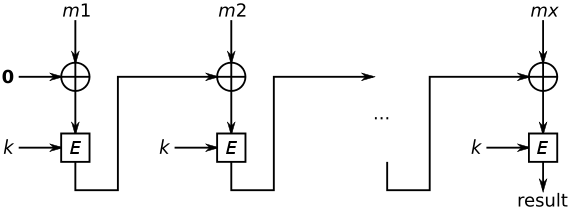
\includegraphics[scale=0.5]{CBC-MAC.png}
\end{figure}

Let's show that $t_{b1c}$ is a valid tag for the message $b||1||(t_b \oplus t_{b'} \oplus c)$
\begin{enumerate}[I.]
\item When we input the $b||1||(t_b \oplus t_{b'} \oplus c)$ the first part of the message is just $b$, while xor-ing with 0 nothing happens, when we will apply the hash function $E$.
\item In the next step we do xor with the second block $1$ and again encode. But what we have so far is the same procedure how the $t_{b'}$ was created!
\item In the next step we should have to $x$ the result so far with the next block$$
t_{b'} \oplus (t_b \oplus t_{b'} \oplus c)
$$
But when xor-ing bitsting with itself we obtain zeros which does not change anything while applying xor.
$$
t_b \oplus c
$$
\item In the next step we have to encode the result of the last xor operation, but in the last step we have done the same operation as we had already done for $t_{b1c}$ - so we have shown that the same tag will be valid for our forged message.
\end{enumerate}
\end{document}